\documentclass[tikz,border=2mm]{standalone}
\usetikzlibrary{shapes.geometric}
\begin{document}
	\pagecolor{brown!20}
	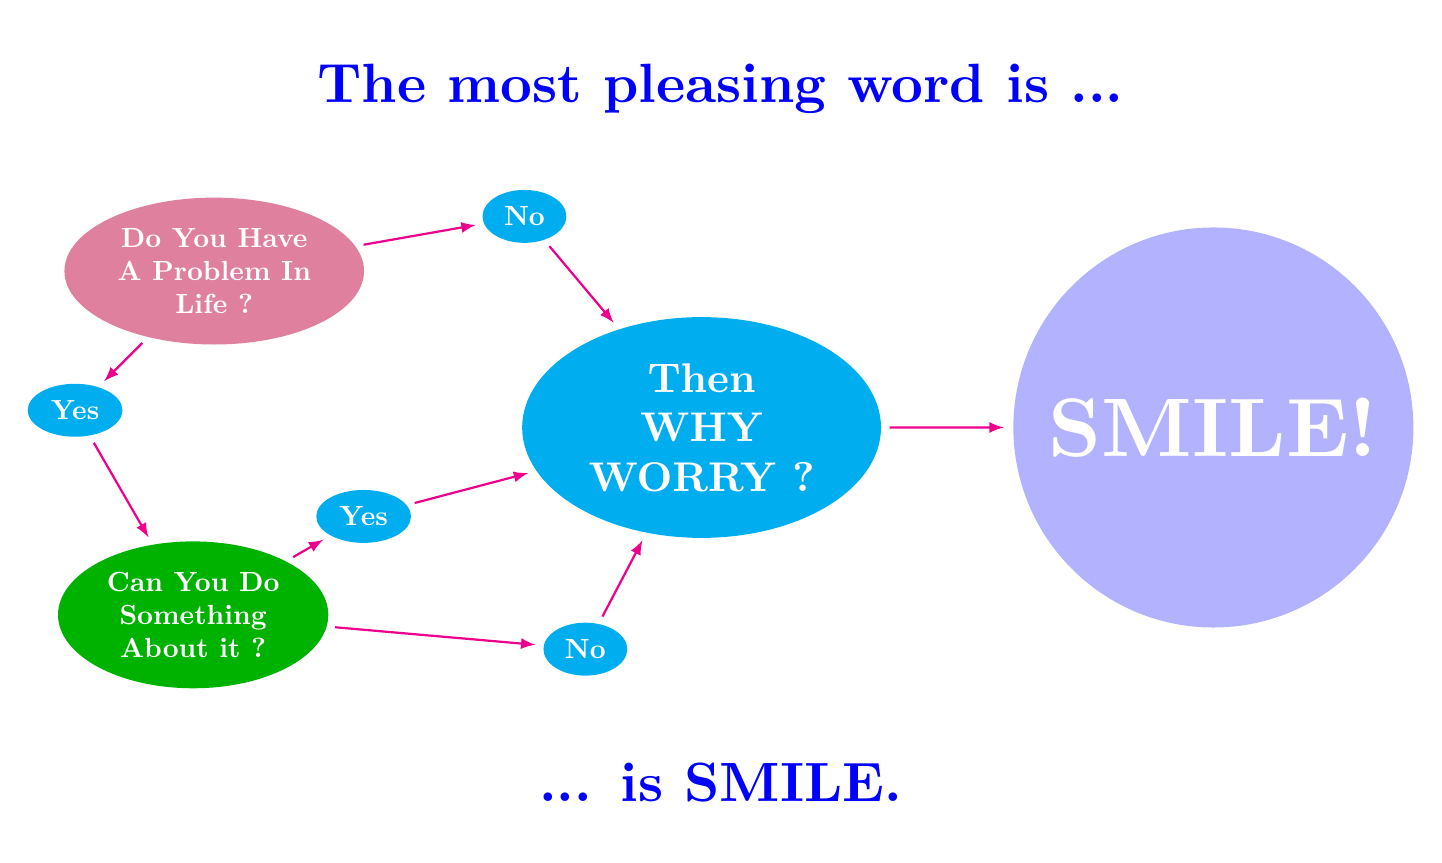
\begin{tikzpicture}
		[every node/.style={ellipse,text=white,font=\bfseries},
		muiten/.style={-latex,magenta,shorten <=1mm,shorten >=1mm,thick}]
		
		\node[fill=purple!50,align=center](A)
		{Do You Have\\A Problem In\\Life ?};
		\path (A) node[shift={(10:4cm)},fill=cyan] (B){No};
		\path (A) node[shift={(-135:2.5cm)},fill=cyan] (C){Yes};
		\path (B) node[shift={(-50:3.5cm)},fill=cyan,scale=1.5,align=center] (D) {Then\\WHY\\WORRY ?};
		\path (C) node[shift={(-60:3cm)},fill=green!70!black,align=center] (E)
		{Can You Do\\ Something\\About it ?};
		\path (E) node[shift={(30:2.5cm)},fill=cyan] (F){Yes};
		\path (E) node[shift={(-5:5cm)},fill=cyan] (G){No};
		\path (D) node[shift={(0:6.5cm)},fill=blue!30,circle,scale=3] (S) {SMILE!};
		
		\draw[muiten] (A)--(B);\draw[muiten] (A)--(C);
		\draw[muiten] (B)--(D);\draw[muiten] (C)--(E);
		\draw[muiten] (E)--(F);\draw[muiten] (E)--(G);
		\draw[muiten] (F)--(D);\draw[muiten] (G)--(D);
		\draw[muiten] (D)--(S);
		
		\draw (current bounding box.north) node[above=5mm,blue,scale=2]
		{The most pleasing word is ...};
		\draw (current bounding box.south) node[below=5mm,blue,scale=2]
		{... is SMILE.};
	\end{tikzpicture}
\end{document}